\subsection{Implementace}

% \begin{framed}
% Implementace or v podmínkách pravidla by vyžadovala výraznou změnu v algoritmu,
% který vytváří síť RETE, neboť join node je problematické znovu využít.
% Implementace forall by vyžadovala změnu vyhodnocování vazeb proměnných a celkově
% join algoritmu. Zvážit problémy implementace všech podobných rozšíření - or,
% and, negace celé konjunkce či disjunkce, exists, forall, viz
% \url{http://www.csie.ntu.edu.tw/~sylee/courses/clips/bpg/node5.4.html}
% \end{framed}

% \begin{framed}
%   \begin{itemize}
%     \item architektura programu (objektový návrh, nedostatky Lispu, je
%       environment jako god class důsledkem těchto problémů?)
%     \item síť RETE, její vytváření $\rightarrow$ výhody - sdílení uzlů
%     \item implementovaná rozšíření
%     \begin{itemize}
%       \item undo/redo - kopie sítě rete, testování ekvivalence
%       \item zpětné řetězení - zásobníky, backtracking, obchází rete
%       \item kompozitní podmínky (not, and, or, forall) - neimplementováno -
%         popsat, jak výrazné změny rete by vyžadovalo a jak by se projevilo na
%         efektivitě (hlavní výhodou rete je sdílení uzlů, které by zde bylo dost
%         problematické)
%       \item syntaktický mód - parser, implementace složených podmínek pro atom
%         (\~{}asdf\&asf) by vyžadovalá podobné změny jako implementace kompozitních
%         podmínek
%       \item gui - capi, propojení s environmentem - notify
%     \end{itemize}
%   \end{itemize}
% \end{framed}

\begin{framed}
  Zmínit použité knihovny - iterate, xlunit
\end{framed}

\subsubsection{Architektura programu}

V následující kapitole budu používat obecný pojem \emph{modul} pro ohraničenou část
programu, implementující nějakou část funkcionality. Veřejné rozhraní modulu
definuje vstupní body, pomocí nichž s ním mohou ostatní moduly komunikovat.
Ty jsou zde reprezentovány funkcemi, makry a metodami, které modul poskytuje
a specifikacemi jejich parametrů. V Common Lispu sice tuto entitu nazýváme
\emph{package}, tento pojem se však špatně skloňuje a celkově narušuje plynulost
textu.

\begin{figure}[h]
\centering
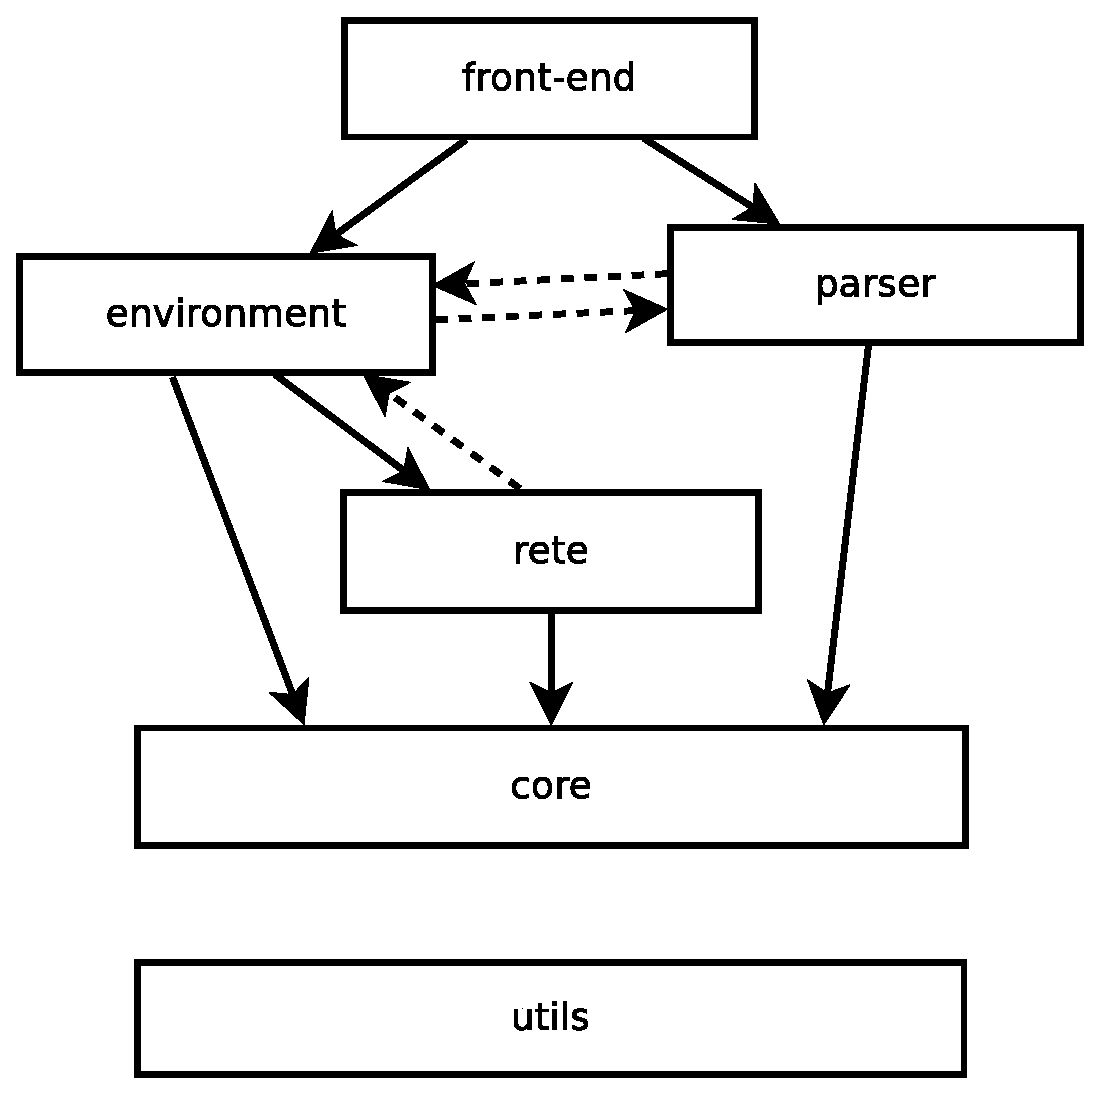
\includegraphics[height=10cm]{modules.eps}
\caption{Architektura ExiLu}
\label{modules}
\end{figure}

Obrázek \ref{modules} zobrazuje architekturu knihovny ExiL, tedy moduly, do
kterých je kód knihovny rozdělen, a jejich vzájemnou komunikaci. Orientace šipek
určuje směr volání funkcí (metod, maker) poskytovaných moduly, např. modul
\verb|front-end| volá funkce modulu \verb|parser| a ne naopak. Těmito voláními
jsou zároveň definovány závislosti mezi moduly, ty mají tedy stejnou orientaci.

Modul \verb|utils| definuje různorodé pomocné funkce a makra, která jsou volána
všemi ostatními moduly. V obrázku \ref{modules} bych tedy mohl zahrnout šipky ze
všech ostatních modulů do modulu \verb|utils|, to by jej však činilo zbytečně
nepřehledným. Většina funkcí a maker, která modul definuje, usnadňuje
nízkoúrovňovou práci se symboly a datovými strukturami - (asociativními)
seznamy, množinami, stromy, \emph{hashovacími tabulkami} apod.

Modul \verb|core| definuje základní objekty, s nimiž zbytek knihovny
pracuje. Ty reprezentují fakty, vzory, šablony a pravidla. Fakty a vzory jsou
definovány ve dvou variantách - jednoduché a strukturované, jak jsem uvedl v
uživatelské příručce.

Modul \verb|rete| implementuje algoritmus RETE, který slouží k efektivnímu
vyhodnocování podmínek odvozovacích pravidel. Algoritmus je implementován
\emph{dataflow} sítí, jejíž fungování popíšu detailně v kapitole \ref{rete}
Algoritmus RETE je sice nejkomplexnější částí ExiLu, veřejné rozhraní modulu
\verb|rete| je však velmi jednoduché.

Modul poskytuje dvojici metod, kterými síť RETE upozorníme na přidání nebo
odebrání pravidel. Ty dle potřeby doplní síť o uzly potřebné k vyhodnocení
podmínek těchto pravidel, případně uzly při odebrání pravidla odstraní.

Další dvojice metod upozorní síť na přidání faktu do (resp. odebrání z) pracovní
paměti. Síť pak přepočítá splněné podmínky pravidel a případně upozorní
prostředí na nově přibyvší nebo rozbité shody (\emph{broken match} - pravidla,
která byla splněná nějakou posloupností faktů a už nejsou).

Modul \verb|environment| definuje stejnojmenný objekt, který udržuje průbežný
stav prostředí a řídí průběh inference. Hodnoty, které stav prostředí tvoří,
jsem popsal v kapitole \ref{env cleanup} Prostředí udržuje krom jiného
referenci na síť \verb|rete|, kterou upozorňuje na nastalé změny.

Modul \verb|parser| zajišťuje vytváření \verb|core| objektů z externí
reprezentace (té, kterou předáváme funkcím a makrům při práci s knihovnou).
Modul rozpoznává jak základní, tak CLIPSovou syntax, takže o to, kterou z nich
uživatel používá, se zbytek kódu nemusí dále starat.

Při parsování strukturovaných faktů či vzorů se \verb|parser| dotazuje
aktuálního prostředí na definici šablony. Při zpětné inferenci prostředí
vyhodnocuje volání \verb|assert| v důsledcích pravidel a žádá \verb|parser| o
zparsování reprezentací faktů v~nich. Proto jsem mezi moduly \verb|environment|
a \verb|parser| přidal šrafované šipky. Kromě těchto nutných interakcí spolu
však moduly nekomunikují.

Modul \verb|front-end| udržuje seznam definovaných prostředí a ví, které je
právě aktivní. Kromě manipulace tohoto seznamu modul sám žádnou funkcionalitu
neimplementuje. Pouze kvotuje parametry předané makrům, předává je
\verb|parser|u a~výsledné objekty (se zbytkem parametrů) pak aktivnímu prostředí.

Do diagramu jsem nezahrnul modul \verb|gui|. Ten implementuje grafické
uživatelské rozhraní a poskytuje dvě metody - \verb|show-gui| a
\verb|update-lists|. Rozhraní se dotazuje prostředí, se kterým je svázáno, na
hodnoty aktuálního stavu a je jím upozorněno, pokud se tyto změní.

\subsubsection{Algoritmus RETE}
\label{rete}

Algoritmus RETE slouží k efektivnímu vyhodnocování splnění podmínek odvozovacích
pravidel (dále jen vyhodnocování). Je implementován dataflow sítí. Ta je
rozdělena do dvou částí, označovaných jako alpha a beta. Alpha část sítě
vyhodnocuje splnění jednotlivých podmínek pravidla fakty nově přidanými do či
odebranými z pracovní paměti. Beta část pak zajišťuje zachování konzistence
vazeb proměnných mezi podmínkami.

To, že je vyhodnocování sítí RETE tak efektivní, je zajištěno maximálním
sdílením častí sítě mezi pravidly. Mají-li dvě pravidla strukturálně stejný vzor
nějaké podmínky (liší se jen použité proměnné), sdílí tato pravidla část alpha
sítě, která tuto podmínku vyhodnocuje. Pokud mají dvě pravidla stejných několik
prvních podmínek, sdílí tato pravidla kromě části alpha sítě i část beta sítě,
která zajišťuje konzistenci vazeb proměnných mezi nimi.

Dataflow síť je tvořena uzly. Jejich vzájemné interakce nazýváme
v~algoritmu aktivacemi. Každý uzel má několik sousedů. Aktivace však v síti
probíhají jen jedním směrem. Uzly, které jsou daným uzlem aktivovány, budu
nazývat jeho potomky. Uzly rozdělujeme na dva základní typy - paměťové a
testovací. Paměťové uzly ukládají průběžné výsledky vyhodnocování. Testovací
uzly provádějí různé typy testů (v závislosti na typu uzlu), nutných pro
vyhodnocení podmínek pravidla.  Uzlu je při aktivaci vždy předána nějaká datová
struktura. Tou je buď fakt, nebo token, který reprezentuje posloupnost faktů.
Zatímco paměťové uzly po aktivaci a uložení datové struktury do své paměti vždy
aktivují své potomky, testovací uzly aktivují potomky jen v případě úspěšného
testu.

\begin{figure}[h]
\centering
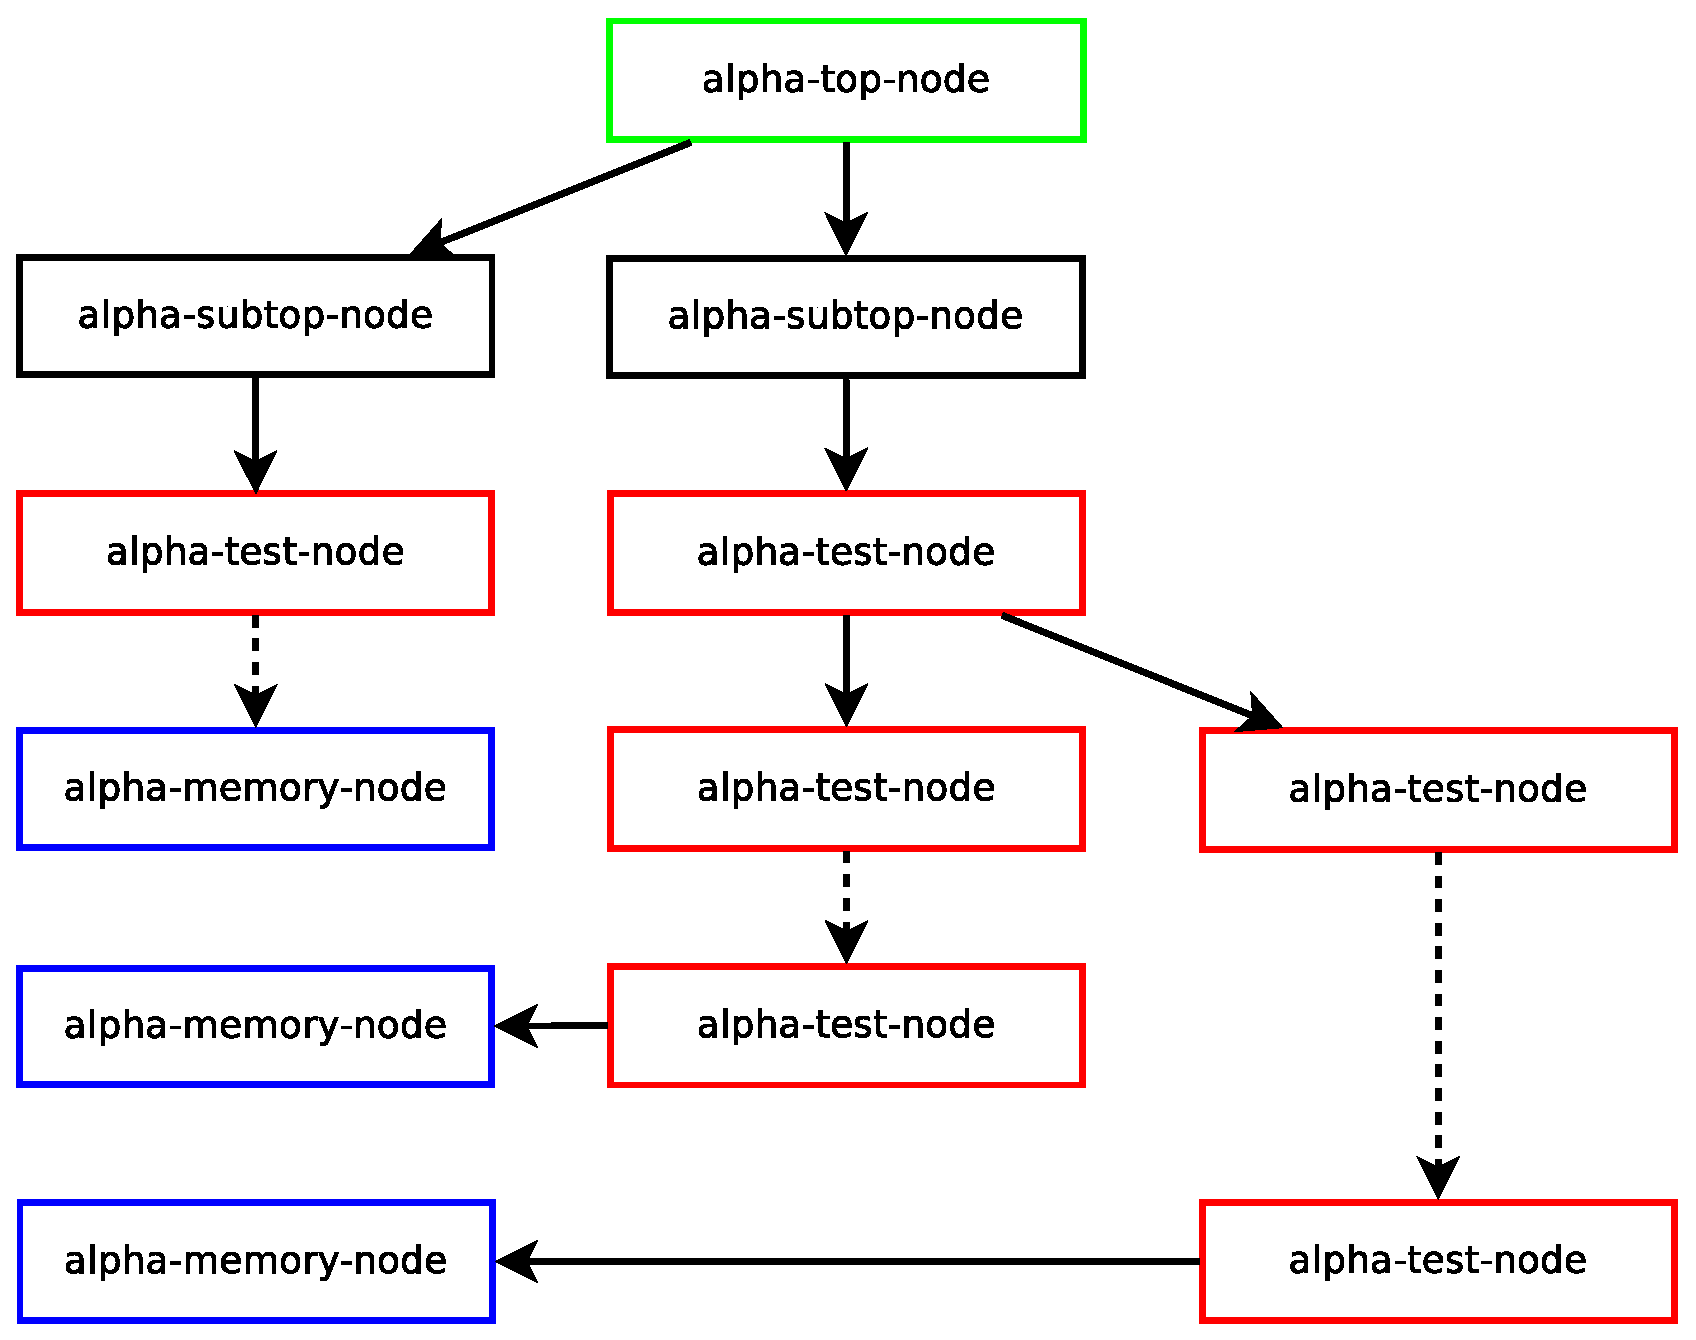
\includegraphics[height=10cm]{rete-alpha.eps}
\caption{Alpha část sítě RETE}
\label{rete-alpha}
\end{figure}

Obrázek \ref{rete-alpha} zobrazuje úsek alpha části sítě RETE. Uzel
\verb|alpha-top-node| je vstupním bodem této sítě. Ten je aktivován při každé
změně pracovní paměti faktem, který byl přidán nebo odebrán. Potomky
\verb|alpha-top-nodu| jsou \verb|alpha-subtop-nody|, jeden pro jednoduché fakty
a jeden pro každou definovanou šablonu. \verb|alpha-top-node| aktivuje příslušný
\verb|alpha-subtop-node| podle typu faktu.

Každá cesta z \verb|alpha-subtop-nodu| do \verb|alpha-memory-nodu| skrze
posloupnost \verb|alpha-test-nodů| vyhodnocuje jednu podmínku nějakého pravidla
(případně skupiny pravidel). Mějme např. pravidla
\begin{minted}{cl}
(defrule rule1
  (in :object box :location ?locaction)
  =>
  ...)
(defrule rule2
  (in :object box :location ?loc)
  =>
  ...).
\end{minted}
Tato pravidla mohou sdílet část alpha sítě pro vyhodnocení svých podmínek, neboť
ty se liší pouze názvy proměnných. Pro vyhodnocení těchto podmínek budeme
potřebovat jeden \verb|alpha-subtop-node| pro šablonu \verb|in|, jeden
\verb|alpha-test-node| pro testování, zda je hodnota slotu \verb|object| rovna
hodnotě \verb|box| a jeden \verb|alpha-memory-node| pro uložení faktů, které
tuto podmínku splňují. Pro slot \verb|location| \verb|alpha-test-node|
nepotřebujeme, neboť alpha část sítě se hodnotami proměnných nezabývá.

\begin{figure}[h]
\centering
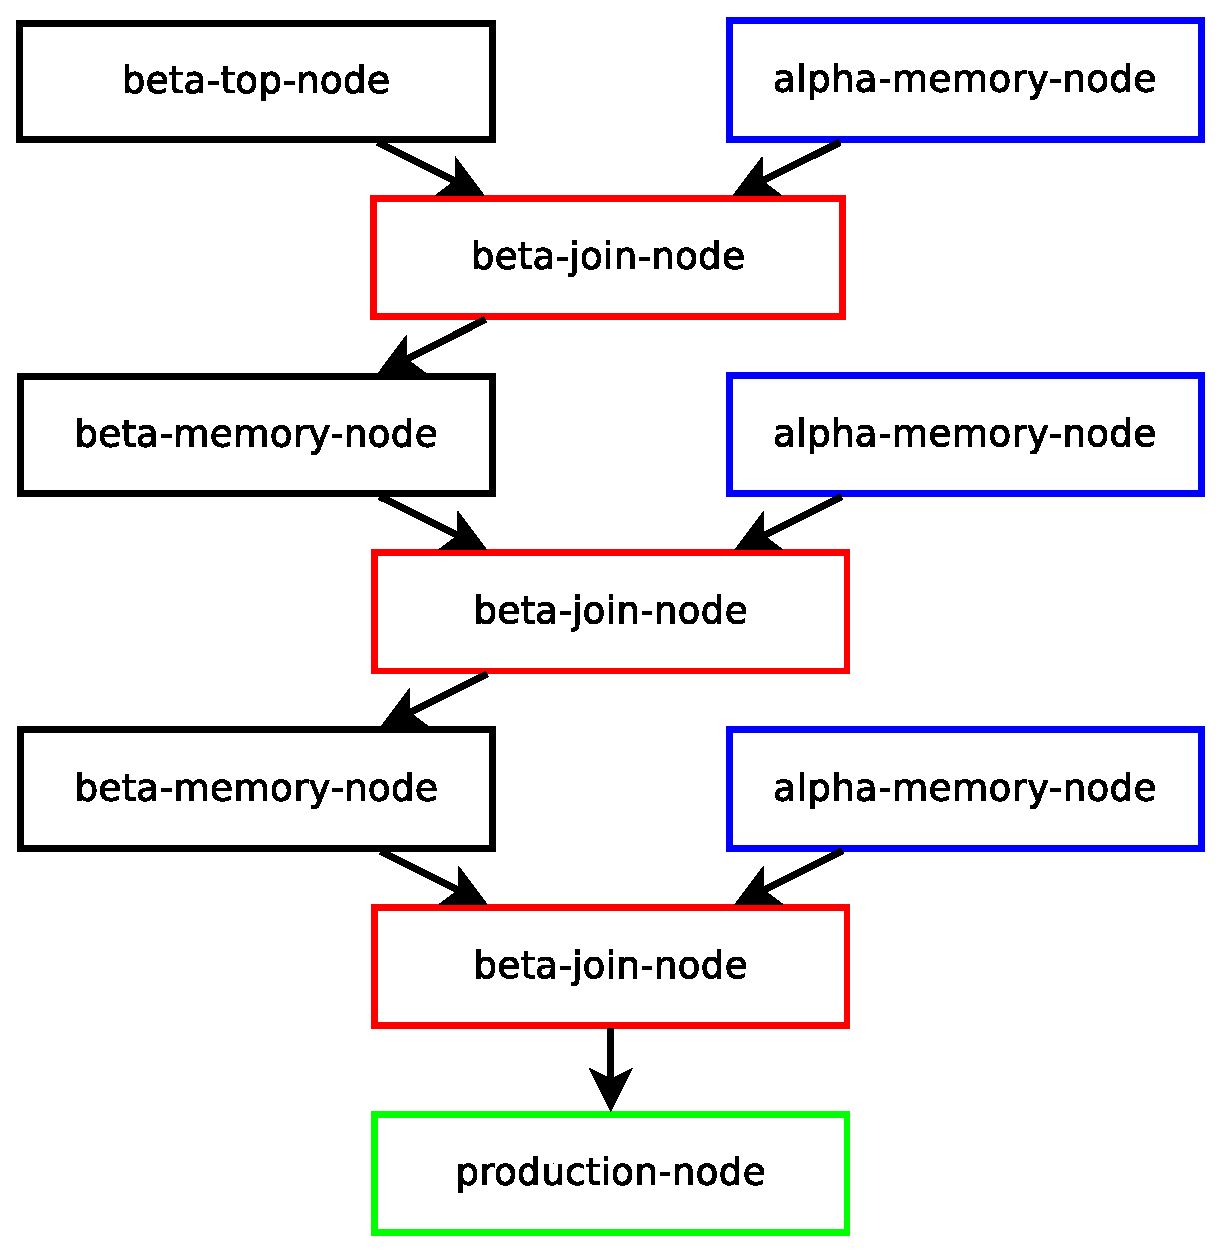
\includegraphics[height=10cm]{rete-beta.eps}
\caption{Beta část sítě RETE}
\label{rete-beta}
\end{figure}

Obrázek \ref{rete-beta} zobrazuje úsek beta části sítě, spolu s
\verb|alpha-memory-nody|, kterými sem vstupují fakta splňující jednotlivé
podmínky pravidel. Každý \verb|beta-memory-node| udržuje množinu tokenů
reprezentujících posloupnosti faktů, z nichž každý splňuje podmínku nějakého
pravidla. \verb|beta-join-nody| pak testují konzistenci vazeb proměnných mezi
těmito podmínkami. \verb|beta-top-node| je speciální případ
\verb|beta-memory-nodu|, který udržuje v paměti pouze jeden prázdný token.
\verb|production-node| je pak speciální případ \verb|beta-memory-nodu|, který
při aktivaci upozorní prostředí, že byly splněny všechny podmínky pravidla,
případně že po odstranění faktu už nejsou všechny splněny.

Mějme například pravidlo
\begin{minted}[samepage]{cl}
(defrule rule
  (goal :object ?obj :from ?from :to ?to)
  (in :object ?obj :location ?from)
  (in :object robot :location ?to)
  =>
  ...).
\end{minted}
Alpha část sítě pro toto pravidlo bude obsahovat tři \verb|alpha-memory-nody|,
každý pro jednu jeho podmínku (kdyby však byla v poslední podmínce místo hodnoty
\verb|robot| proměnná, vystačili bychom si se dvěma \verb|alpha-memory-nody|).

Beta část sítě bude vypadat tak, jako na obrázku \ref{rete-beta}
První (shora) \verb|beta-test-node| ve skutečnosti nemá co testovat, neboť jde o
první podmínku pravidla. První \verb|beta-memory-node| bude udržovat tokeny
délky 1 reprezentující \uv{posloupnost} faktů, které splňují první podmínku.
Druhý \verb|beta-join-node| bude testovat konzistenci vazeb mezi druhou
a první podmínkou pravidla. Druhý \verb|beta-memory-node| bude udržovat tokeny
délky 2 reprezentující dvojice faktů, splňující první dvě podmínky pravidla.
Třetí \verb|beta-join-node| bude testovat konzistenci vazeb mezi třetí podmínkou
pravidla a předchozími dvěma. \verb|production-node| pak bude udržovat tokeny
délky 3 reprezentující trojice faktů splňující všechny podmínky pravidla.

% Druhý \verb|beta-test-node| je aktivován buď zleva \verb|alpha-memory-nodem|,
% přibyde-li fakt, který splňuje druhou podmínku pravidla, nebo zprava
% \verb|beta-memory-nodem|, přibyde-li fakt, který splňuje první podmínku.

Přidávejme nyní postupně fakty do pracovní paměti. Přidáním
\verb|(in :object box :location A)| dojde (po průchodu alpha částí sítě) k
aktivaci druhého \verb|alpha-memory-nodu|. Ten uloží fakt do své paměti
a aktivuje \uv{zprava} druhý \verb|beta-join-node|. Ten prohledá paměť
\verb|beta-memory-nodu| nad sebou, zda neobsahuje nějaký token s
konzistentními vazbami proměnných. Ta je ale prázdná, takže zde se aktivace
zastaví.

Přidáním \verb|(goal :object box :from A :to B)| dojde k aktivaci prvního
\verb|alpha-memory-nodu|. Ten po uložení faktu aktivuje první
\verb|beta-join-node|. Ten nemá co testovat, takže aktivuje
\verb|beta-memory-node| pod sebou. Ten uloží jednoprvkový token s přidaným
faktem a aktivuje opět druhý \verb|beta-join-node|, tentokrát však \uv{zleva}.
\verb|beta-join-node| tentokrát prohledá obsah paměti \verb|alpha-memory-nodu|
nad sebou, zda neobsahuje fakt konzistentní s tokenem. \verb|beta-join-node| zde
testuje, zda jsou hodnoty slotů \verb|object| a \verb|location| faktu v alpha
paměti shodné s hodnotami \verb|object| a \verb|from| prvního faktu tokenu v
beta paměti.

Test zde skončí úspěšně, takže druhý \verb|beta-join-node| aktivuje
\verb|beta-memory-node| pod sebou a předá mu dvouprvkový token s oběma fakty.
Ten aktivuje třetí \verb|beta-join-node| \uv{zleva}. Ten následně prohledá paměť
\verb|alpha-memory-nodu| nad sebou. Ta je ale prázdná, takže zde aktivace skončí.

Po přidání faktu \verb|(in :object robot :location B)| dojde k aktivaci třetího
\verb|alpha-memory-nodu|. Ten fakt uloží a aktivuje třetí \verb|beta-join-node|
\uv{zprava}. Ten prohledá paměť \verb|beta-memory-nodu| nad sebou, zda
neobsahuje konzistentní tokeny. Ta obsahuje dvouprvkový token s prvními dvěma
fakty. \verb|beta-join-node| tedy srovná hodnotu slotu \verb|location| přidaného
faktu s hodnotou \verb|to| prvního faktu tokenu. Protože tyto hodnoty se
shodují, aktivuje \verb|beta-join-node| \verb|production-node| pod sebou a předá
mu tříprvkový token s posloupností faktů, které splňují všechny podmínky
pravidla. Ten token uloží a upozorní prostředí, že pravidlo bylo splňeno
posloupností faktů v tokenu.

\subsubsection{Kompozitní podmínky pravidel}

Podporu kompozitních podmínek odvozovacích pravidel (vnořené aplikace logických
funkcí v podmínkách) jsem v ExiLu neimplementoval. Rád bych zde ale ukázal, proč
je implementace této funkcionality vzhledem k aktuální implementaci algoritmu
RETE složitá.

\begin{figure}[h]
\centering
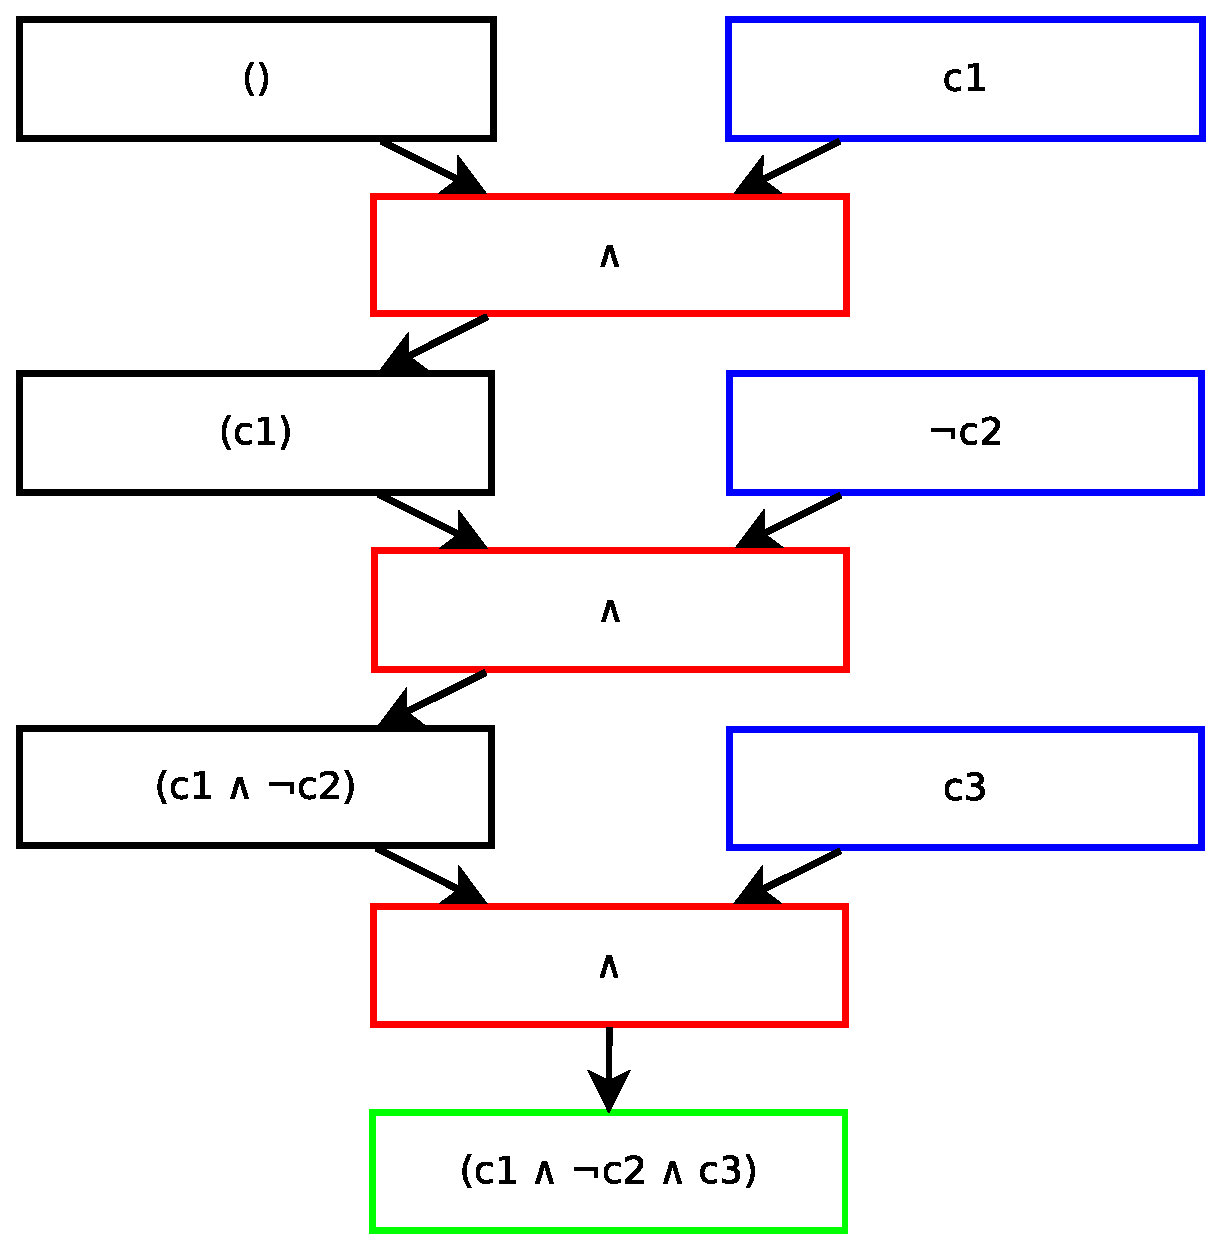
\includegraphics[height=10cm]{rete-beta-conds.eps}
\caption{Beta část sítě RETE s funkcemi uzlů}
\label{rete-beta-conds}
\end{figure}

Obrázek \ref{rete-beta-conds} ukazuje diagram beta části sítě RETE z předchozí
sekce. Názvy uzlů jsem zde ale nahradil jejich funkcí. Paměťové uzly ukládají
fakty nebo tokeny splňující jednu (v případě alpha-memory-nodů), nebo více (u
beta-memory-nodů) podmínek pravidla. Testovací (beta-join-nody) pak zajišťují
agregaci těchto faktů a tokenů. Jednu z podmínek jsem navíc pro ukázku znegoval.

Síť v diagramu splňuje několik podmínek:
\begin{enumerate}
  \item uzly jsou konstruovány ve stejném pořadí, v jakém se podmínky v definici
    pravidla vyskytují,
  \item beta-join-node vždy spojuje jeden alpha-memory-node s jedním
    beta-memory-nodem, agreguje tedy fakty splňující jednu podmínku pravidla s
    tokeny reprezentujícími posloupnost faktů splňující jeho předchozí podmínky,
  \item negace podmínky je vždy aplikována jen na úrovni jednoho faktu.
\end{enumerate}

\begin{figure}[h]
\centering
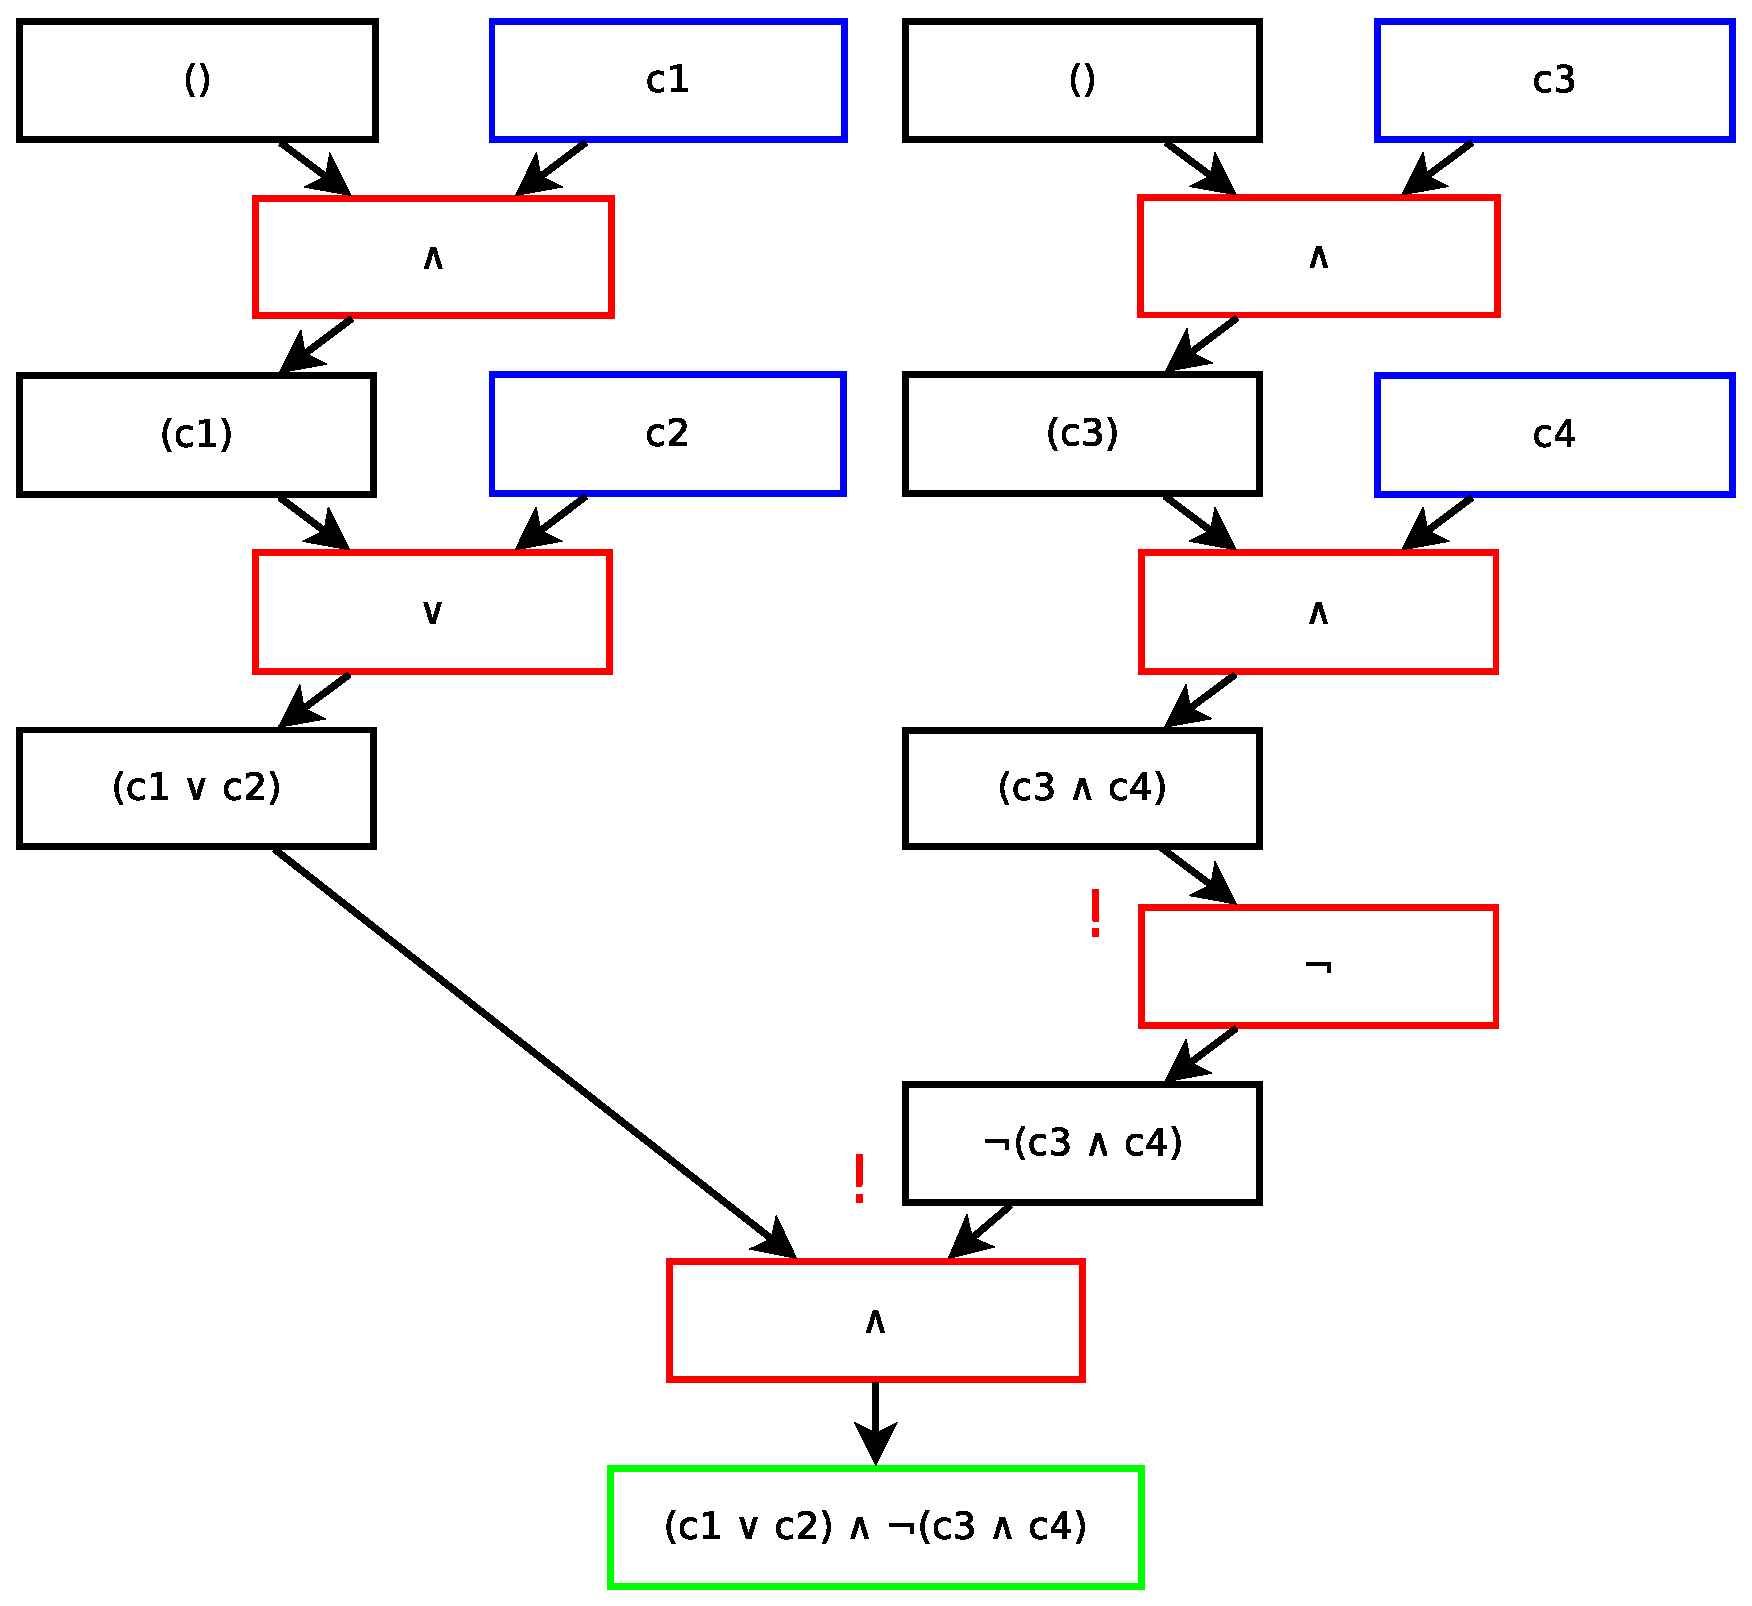
\includegraphics[height=12cm]{rete-beta-comp-conds.eps}
\caption{Síť RETE s kompozitními podmínkami}
\label{rete-beta-comp-conds}
\end{figure}

Představme si nyní stavbu RETE sítě v případě následujícícho pravidla
s~kompozitními podmínkami:
\begin{minted}{cl}
(defrule rule
  (and (or condition1 condition2)
       (not (and condition3 condition4)))
  =>
  ...)
\end{minted}
Ta je zobrazena na obrázku \ref{rete-beta-comp-conds} Z diagramu vidíme, že síť porušuje všechny
uvedené podmínky.

\begin{framed}
  \begin{itemize}
    \item popsat, co je problematického na podpoře této sítě
    \item podmínky třeba procházet rekurzivně a síť budovat stromovitě
    \item token je nyní list, stačí to, nebo musí být také strom?
    \item testy v join nodech nyní ukládají pozici - o kolik podmínek zpět,
      který atom v přechozí, který atom v aktuální
    \item pozice by musela mít u beta-beta joinu minimálně jednu pozici navíc -
      (fakt,atom)-(fakt,atom), pokud by musel být token strom, ještě složitější
    \item lze vyřešit join-nody obecně - beta-beta i beta-alpha, nebo nutné dva
      typy?
    \item jak reprezentovat node, který neguje složenou podmínku?
    \item jak joinovat tokeny, které mohou zahrnovat výsledky negativní podmínky?
    \item síť je cyklická a jako taková špatně vizualizuje
    \item počet uzlů sítě roste velmi rychle $\rightarrow$ mnoho uzlů i při
      několika pravidlech $\rightarrow$ náročné ladění
    \item podpora kompozitních podmínek je navíc problematická vzhledem ke
      zpětné inferenci (ale ta už je stejně omezená) - znamenalo by složené cíle
      (kvůli or, not)
    \item zmínit, jak jednoduchá je implementace, pokud podmínky pracují pouze
      se substitucemi proměnných - bez rete
  \end{itemize}
\end{framed}
% Z fungování beta částí sítě RETE (viz sekce \ref{rete}) vidíme, že vyhodnocování
% podmínek pravidla je inherentně sekvenční. \verb|Beta-join-nody| zde
% implementují logickou spojku \emph{a} mezi podmínkami pravidla, která je zde
% zleva asociativní.

\subsubsection{Undo/redo}
Možnost vrácení provedených akcí a jejich opětovného provedení (undo/redo) je
implementována na úrovni prostředí, které udržuje aktuální stav systému.
Hodnoty, které stav tvoří, jsem popsal v sekci \ref{env cleanup} a možnosti,
které undo/redo poskytuje, v sekci \ref{undo}

Prostředí je v programu reprezentováno objektem \verb|environment|. Stav
prostředí je uchováván ve slotech tohoto objektu.

Prostředí dále udržuje dva zásobníky - \verb|undo| a \verb|redo|.
Každý z~těchto zásobníků ukládá seznamy tvořené popiskem akce k vrácení,
uzávěrem, který akci vrátí a~uzávěrem, který ji opět provede. První uzávěr ve
svém lexikálním prostředí uchovává hodnoty potřebné k vrácení akce. Zásobníky
jsou manipulovány pouze několika makry a metodami k tomu určenými, zbytek kódu k
zásobníkům přímo nepřistupuje.

Tělo každé akce, která mění hodnoty prostředí, je obaleno buď voláním makra
\verb|with-undo|, nebo \verb|with-saved-slots|. Volání \verb|with-undo| je kromě
těla akce předán uzávěr, který zajistí její vrácení. Makro \verb|with-undo|
po vyhodnocení těla akce zajistí, že se na zásobník \verb|undo| uloží předaný
uzávěr spolu s uzávěrem, který akci opět provede při volání \verb|redo|.
Tento druhý uzávěr pouze vyhodnotí původní tělo akce.

Makro \verb|with-saved-slot| zjednodušuje volání \verb|with-undo|. Toto makro
bere kromě těla akce seznam slotů prostředí, které je třeba před akcí uložit.
Makro pak automaticky vytvoří uzávěr, který předá makru \verb|with-undo|. Tento
uzávěr si ve svém lexikálním prostředí pamatuje kopie původních hodnot požadovaných
slotů prostředí a při vyhodnocení je nastaví zpět na tyto hodnoty.

Prostředí ke každému svému slotu definuje metodu \verb|copy-<slot>|, např.
\verb|copy-facts|. Makro \verb|with-saved-slots| tedy vytvoří potřebný uzávěr
tak, že v \verb|let|u naváže výsledky volání těchto metod pro každý požadovaný
slot. V tomto \verb|let|u pak vytvoří anonymní (lambda) funkci, která hodnoty
prostředí nastaví zpět na ty, které \verb|let| navázal.

Funkce \verb|undo| pak jednoduše odstraní seznam z vrcholu zásobníku
\verb|undo|, zavolá uzávěr, který vrátí poslední akci a druhý uzávěr, který akci
opět provede, uloží na vrchol zásobníku \verb|redo|. Funkce \verb|redo| funguje
symetricky.

Nakonec je třeba zajistit, aby každé volání \verb|with-undo| uložilo na zásobník
právě jeden uzávěr k vrácení akce. Například pokud samostatně voláme makro
\verb|assert| pro přidání nějakého faktu do pracovní paměti, chceme, aby toto volání
bylo možné vrátit. Pokud ale voláme \verb|step|, jehož výsledkem je aktivace
nějakého pravidla, které ve svých důsledcích volá makro \verb|assert|, chceme,
aby se volání \verb|step| uložilo na zásobník jako jedna akce. Volání
\verb|assert|, ke kterému v průběhu této akce dojde, už samostatně ukládat
nechceme.

K tomuto účelu definuje prostředí dynamickou proměnnou \verb|*undo-enabled*|.
Makro \verb|with-undo| ukládá uzávěr na zásobník jen v případě, že je hodnota
této proměnná \verb|true|. Tělo akce pak makro vyhodnocuje s hodnotou této
proměnné navázanou na \verb|false|. Tím je zajištěno, že se uzávěr na zásobník
\verb|undo| uloží vždy jen v \uv{nejvnějšnějším} volání makra \verb|with-undo|.

Díky makrům \verb|with-undo| a \verb|with-saved-slots| je možné velmi snadno
přidat do prostředí další akce s možností jejich vrácení. Stačí jen tělo akce
obalit jedním z těchto maker bez nutnosti vědět, jak je vrácení akce
implementováno. Pokud potřebujeme do prostředí přidat další slot, jehož hodnotu
je třeba při volání \verb|undo| obnovovat, stačí k tomuto slotu implementovat
metodu \verb|copy|.

Nejsložitějším problémem při implementaci vracení akcí bylo implementovat metodu
\verb|copy-rete|. Ta kopíruje dataflow síť RETE uloženou ve slotu \verb|rete|
prostředí. Kopírovnání sítě RETE je složité, neboť síť obsahuje cykly. Síť se
sice z~pohledu aktivace uzlů chová jako acyklický graf, některé uzly však
uchovávájí reference na své sousedy proti směru hran tohoto grafu.

Pro účely kopírování sítě RETE jsem implementoval obecnou metodu vyššího řádu
pro průchod cyklickým grafem. Tato metoda využívá techniky
memoizace\footnote{\url{http://en.wikipedia.org/wiki/Memoization}}. Metoda bere
kromě výchozího uzlu grafu tři funkce, které aplikuje na navštěvované uzly před
memoizací a jimiž zajišťuje agregaci hodnot vrácených sousedy uzlu.

Fungování metody je pro textový popis příliš složité, považuji ji však za jednu
z nejzajímavějších částí nového kódu, hlavně díky její obecnosti. Zrojový kód
metody je v souboru \verb|rete/graph-traversal.lisp|, kód kopírující síť rete,
který metodu využívá pak v souboru \verb|rete/rete-copy.lisp|. Celkově je kód
zajišťující kopírování sítě RETE asi třikrát delší, než zbytek kódu
implementující funkcionalitu undo/redo.


\subsubsection{Zpětné řetězení}
\subsubsection{CLIPSová syntax}
\subsubsection{Grafické uživatelské rozhraní}
